% -*- latex -*-
%%%%%%%%%%%%%%%%%%%%%%%%%%%%%%%%%%%%%%%%%%%%%%%%%%%%%%%%%%%%%%%%
%%%%%%%%%%%%%%%%%%%%%%%%%%%%%%%%%%%%%%%%%%%%%%%%%%%%%%%%%%%%%%%%
%%%%
%%%% This text file is part of the source of 
%%%% `The Art of HPC, vol 1: The Science of Computing'
%%%% by Victor Eijkhout, copyright 2012-2023
%%%%
%%%% This book is distributed under a Creative Commons Attribution 3.0
%%%% Unported (CC BY 3.0) license and made possible by funding from
%%%% The Saylor Foundation \url{http://www.saylor.org}.
%%%%
%%%%
%%%%%%%%%%%%%%%%%%%%%%%%%%%%%%%%%%%%%%%%%%%%%%%%%%%%%%%%%%%%%%%%
%%%%%%%%%%%%%%%%%%%%%%%%%%%%%%%%%%%%%%%%%%%%%%%%%%%%%%%%%%%%%%%%

\index{arithmetic!computer|see{floating point arithmetic}}
\index{computer arithmetic|see{floating point arithmetic}}
\index{floating point arithmetic|(textbf}

Of the various types of data that one normally encounters, the ones we
are concerned with in the context of scientific computing are the
numerical types: integers (or whole numbers)
$\ldots,-2,-1,0,1,2,\ldots$, real numbers $0,1,-1.5,2/3,\sqrt 2,\log
10,\ldots$, and complex numbers $1+2i,\sqrt 3-\sqrt 5i,\ldots$.
Computer hardware is organized to give only a certain amount of space to
represent each number, in multiples of bytes, each
containing 8~bits. Typical values are 4 bytes for an
integer,  4~or~8 bytes for a real number, and 8~or~16 bytes for a
complex number.

Since only a certain amount of memory is available to store a number,
it is clear that not all numbers of a certain type can be stored. For
instance, for integers only a range is stored.
%
(Languages such as
\emph{Python}\index{Python!large integers}
have arbitrarily \emph{large integers}, but this has no hardware support.)
%
In the case of real
numbers, even storing a range is not possible since any interval $[a,b]$
contains infinitely many numbers. Therefore, any
\indextermsub{representation of}{real numbers} will cause gaps between the
numbers that are stored. 
Calculations in a computer are sometimes
described as \indextermsub{finite precision}{arithmetic},
to reflect that in general you not store numbers with infinite
precision.

Since many results are not representable, any computation that results in
such a number will have to be dealt with by issuing an
error or by approximating the result. 
In this chapter we will look at
how finite precision is realized in a computer,
and
the ramifications of such approximations of the `true' outcome of
numerical calculations. 

For detailed discussions,
\begin{itemize}
\item the ultimate reference to floating point arithmetic
  is the \indexterm{IEEE 754} standard~\cite{754-2019};
\item for secondary reading,
  see the book by
  Overton~\cite{Overton:754book}; it is easy to find online copies of
  the essay by Goldberg~\cite{goldberg:floatingpoint};
\item for extensive
  discussions of round-off error analysis in algorithms, see the books
  by Higham~\cite{Higham:2002:ASN} and Wilkinson~\cite{Wilkinson:roundoff}.
\end{itemize}

\Level 0 {Bits}
\label{sec:bits}

At the lowest level, computer storage and computer numbers
are organized in \indextermdef{bit}s.
A~bit, short for `binary digit', can have the values zero and one.
Using bits we can then express numbers in \indextermdef{binary} notation:
\begin{equation}
  \mathtt{10010}_2 \equiv \mathtt{18}_{10}
\end{equation}
where the subscript indicates the base of the number system,
and in both cases the rightmost digit is the least significant one.

The next organizational level of memory is the \indextermdef{byte}:
a~byte consists of eight bits, and can therefore represent
the values~$0\cdots 255$.

\begin{exercise}
  %{Bit operations}
  \label{ex:bit-even}
  Use bit operations to test whether a number is odd or even.\\
  Can you think of more than one way?
\end{exercise}

\Level 0 {Integers}
\label{sec:int-rep}

In scientific computing, most operations are on real
numbers. Computations on integers rarely add up to any serious
computation load, except in applications such as cryptography.
There are also applications such as `particle-in-cell' that
can be implemented with bit operations.
However, integers are still encountered in indexing calculations.

Integers are commonly stored in 16, 32, or 64~bits, with 16 becoming
less common and 64 becoming more and more so. The main reason for this increase is
not the changing nature of computations, but the fact that integers
are used to index arrays. As the size of data sets grows (in
particular in parallel computations), larger indices are needed. For
instance, in 32~bits one can store the numbers zero through
$2^{32}-1\approx 4\cdot 10^9$. In other words, a 32 bit index can
address 4 gigabytes of memory. Until recently this was enough for most
purposes; these days the need for larger data sets has made 64~bit
indexing necessary.

When we are indexing an array, only positive integers are needed.
In general integer computations, of course, we need to accommodate
the negative integers too. We will now discuss several strategies for
implementing negative integers. Our motivation here will be that
arithmetic on positive and negative integers should be as simple as on
positive integers only: the circuitry that we have for comparing and
operating on bitstrings should be usable for (signed) integers.

There are several ways of implementing
negative integers. The simplest solution is to reserve one bit as a
\indexterm{sign bit}, and use the remaining 31 (or 15 or 63; from now on we will
consider 32 bits the standard) bits to store the
absolute magnitude. By comparison, we will call the straightforward
interpretation of bitstrings as \indexterm{unsigned} integers.

\begin{equation}
\begin{array}{crrrrrr}
  \toprule
  \hbox{bitstring}&
  00\cdots0&\ldots&01\cdots1&
  10\cdots0&\ldots&11\cdots1\\ \midrule
  \hbox{interpretation as unsigned int}&
  0&\ldots&2^{31}-1&
  2^{31}&\ldots&2^{32}-1\\ \midrule
  \hbox{interpretation as signed integer}&
  0&\cdots&2^{31}-1&
  -0&\cdots&-(2^{31}-1)\\
  \bottomrule
\end{array}
\end{equation}

This scheme has some disadvantages, one being that
there is both a positive and negative number zero. This means that a test
for equality becomes more complicated than simply testing for equality
as a bitstring. More importantly, in the second half of the
bitstring, the interpretation as signed integer decreases,
going to the right. This means that a test for greater-than becomes
complex; also
adding a positive number to a
negative number now has to be treated differently from adding it to a
positive number.

Another solution would be to let an unsigned number $n$ be interpreted
as $n-B$ where $B$ is some plausible bias, for instance~$2^{31}$.

\begin{equation}
\begin{array}{crrrrrr}
  \toprule
  \hbox{bitstring}&
  00\cdots0&\ldots&01\cdots1&
  10\cdots0&\ldots&11\cdots1\\ \midrule
  \hbox{interpretation as unsigned int}&
  0&\ldots&2^{31}-1&
  2^{31}&\ldots&2^{32}-1\\ \midrule
  \hbox{interpretation as shifted int}&
  -2^{31}&\ldots&-1&
  0&\ldots&2^{31}-1\\ \bottomrule
\end{array}
\end{equation}

This shifted scheme does not suffer from the $\pm0$ problem, and
numbers are consistently ordered. However, if we compute $n-n$
by operating on the bitstring that represents~$n$, we do not 
get the bitstring for zero.

To ensure this desired behavior,
we instead rotate the number line with positive and negative numbers
to put the pattern for zero back at zero.
The resulting scheme, which is the one that is used most commonly, is
called \indexterm{2's complement}. Using this scheme,
the representation of integers is
formally defined as follows.
\begin{definition}
  Let $n$ be an integer, then the 2's complement `bit pattern'
  $\beta(n)$ is a non-negative integer defined as follows:
  \begin{itemize}
  \item If $0\leq n\leq 2^{31}-1$, the normal bit pattern for $n$ is
    used, that is
    \begin{equation}
      0\leq n\leq 2^{31}-1 \Rightarrow \beta(n) = n.
    \end{equation}
  \item For $-2^{31}\leq n\leq -1$, $n$ is represented by the bit
    pattern for $2^{32}-|n|$:
    \begin{equation}
      -2^{31}\leq n\leq -1 \Rightarrow \beta(n) = 2^{32}-|n|.
    \end{equation}
  \end{itemize}
  We denote the inverse function that takes a bit pattern and
  interprets as integer with~$\eta=\beta\inv$.
\end{definition}

The following diagram shows the correspondence between bitstrings and
their interpretation as 2's complement integer:
\begin{equation}
\begin{array}{crrrrrr}
  \toprule
  \hbox{bitstring $n$}&
  00\cdots0&\ldots&01\cdots1&
  10\cdots0&\ldots&11\cdots1\\ \midrule
  \hbox{interpretation as unsigned int}&
  0&\ldots&2^{31}-1&
  2^{31}&\ldots&2^{32}-1\\ \midrule
  \hbox{interpretation $\beta(n)$ as 2's comp. integer}&
  0&\cdots&2^{31}-1&
  -2^{31}&\cdots&-1\\
  \bottomrule
\end{array}
\end{equation}

Some observations:
\begin{itemize}
\item There is no overlap between the bit patterns for positive and
  negative integers, in particular, there is only one pattern for zero.
\item The positive numbers have a leading bit zero, the negative
  numbers have the leading bit set.
  This makes the leading bit act like a sign bit; however note the
  above discussion.
\item If you have a positive number~$n$, you get $-n$ by flipping
  all the bits, and adding~1.
\end{itemize}

\begin{exercise}
  \label{ex:compare-mn}
  For the `naive' scheme and the 2's complement scheme for negative
  numbers, give pseudocode for the comparison test $m<n$, where $m$
  and~$n$ are integers. Be careful to distinguish between all cases of
  $m,n$ positive, zero, or negative.
\end{exercise}

\Level 1 {Integer overflow}

Adding two numbers with the same sign, or multiplying two numbers of
any sign, may lead to a result that is too
large or too small to represent. This is called \indexterm{overflow};
see section~\ref{sec:exceptions} for the corresponding floating
point phenomenon.
The following exercise lets you explore the behavior of an actual
program.

\begin{exercise}
  \label{ex:int-overflow}
  Investigate what happens when you perform such a calculation. What
  does your compiler say if you try to write down a non-representable
  number explicitly, for instance in an assignment statement?
\end{exercise}

If you program this in~C, it is worth noting that while you
probably get an outcome that is understandable, the behavior
of overflow in the case of signed quantities is actually
\emph{undefined}\index{C!undefined behavior}
under the C~standard.

\Level 1 {Addition in two's complement}

Let us consider doing some simple arithmetic on 2's complement
integers. We start by assuming that we have hardware that works on unsigned integers.
The goal is to see that we can use this hardware to do calculations
on signed integers, as represented in 2's complement.

We consider the computation of $m+n$, where $m,n$ are representable
numbers:
\begin{equation}
  0\leq |m|,|n|<2^{31}.
\end{equation}
We distinguish different cases.
\begin{itemize}
\item The easy case is $0<m,n$. In that case we perform the normal
  addition, and as long as the result stays under $2^{31}$, we get the
  right result. If the result is $2^{31}$ or more, we have integer
  overflow, and there is nothing to be done about that.
  %
  \begin{figure}[ht]
    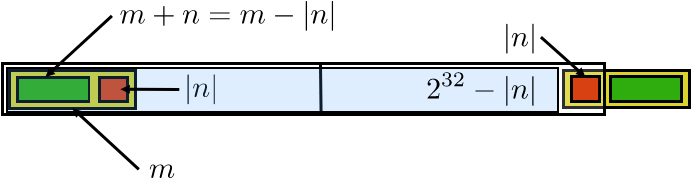
\includegraphics[scale=.5]{mminusn1}
    \caption{Addition with one positive and one negative number in 2's complement.}
    \label{fig:mminusn1}
  \end{figure}
  %
\item Case $m>0$, $n<0$, and $m+n>0$. 
  Then $\beta(m)=m$ and
  $\beta(n)=2^{32}-|n|$, so the unsigned addition becomes
  \begin{equation}
    \beta(m)+\beta(n)=m+(2^{32}-|n|)=2^{32}+m-|n|.
  \end{equation}
  Since $m-|n|>0$, this result is~$>2^{32}$.
  %
  (See figure~\ref{fig:mminusn1}.)
  %
  However, we observe that
  this is basically $m+n$ with the 33rd bit set. If we ignore this
  overflowing bit, we then have the correct result.
\item Case $m>0$, $n<0$, but $m+n<0$. Then
  \begin{equation}
    \beta(m)+\beta(n) = m+ (2^{32}-|n|) = 2^{32}-(|n|-m).
  \end{equation}
  Since $|n|-m>0$ we get
  \begin{equation}
    \eta\bigl(2^{32}-(|n|-m)\bigr) = -\left| (|n|-m) \right| = m-|n|=m+n.
  \end{equation}
\end{itemize}

\Level 1 {Subtraction in two's complement}

In exercise~\ref{ex:compare-mn} above you explored comparing two integers.
Let us now explore how 
subtracting numbers in two's complement is implemented. Consider $0\leq
m\leq 2^{31}-1$ and $1\leq n\leq 2^{31}$ and let us see what happens
in the computation of $m-n$. 

Suppose we have an algorithm for adding and subtracting unsigned
32-bit numbers. Can we use that to subtract two's complement integers?
We start by observing that the integer subtraction $m-n$ becomes the
unsigned addition $m+(2^{32}-n)$.
\begin{itemize}
\item Case: $m<|n|$. In this case, $m-n$ is negative and
  $1\leq |m-n|\leq 2^{31}$, so the bit pattern for $m-n$ is
  \begin{equation}
    \beta(m-n) = 2^{32}-(n-m).
  \end{equation}
  Now, $2^{32}-(n-m)=m+(2^{32}-n)$, so we can compute
  $m-n$ in 2's complement by adding the bit patterns of $m$ and $-n$ as
  unsigned integers:
  \begin{equation}
    \eta\bigl( \beta(m)+\beta(-n) \bigr) =
  \eta\bigl( m+(2^{32}-|n|) \bigr) =
  \eta\bigl( 2^{32} + (m-|n|) \bigr) = 
  \eta\left( 2^{32} - \bigl|m-|n|\bigr| \right) = m-|n| = m+n
  .
  \end{equation}
\item Case: $m>n$. Here we observe that
  $m+(2^{32}-n)=2^{32}+m-n$. Since $m-n>0$, this is a number $>2^{32}$
  and therefore not a legitimate
  representation of a negative number. However, if we store this
  number in 33 bits, we see that it is
  the correct result $m-n$, plus a single bit in the
  33-rd position. Thus, by performing the unsigned addition, and
  ignoring the \indexterm{overflow bit}, we again get the correct result.
\end{itemize}
In both cases we conclude that we can perform the subtraction $m-n$ by adding
the unsigned number that represent $m$ and $-n$
and ignoring overflow if it occurs.

\Level 1 {Binary coded decimal}
\label{sec:bcd}

Decimal numbers are not relevant in scientific computing, but they are
useful in financial calculations, where computations involving money
absolutely have to be exact. Binary arithmetic is at a disadvantage
here, since numbers such as $1/10$ are repeating fractions in
binary. With a finite number of bits in the mantissa\index{mantissa},
this means that the number $1/10$ can not be represented exactly in
binary.  For this reason, \indexterm{binary-coded-decimal} schemes
were used in old IBM\index{IBM} mainframes, and are in fact being
standardized in revisions of \indexterm{IEEE 754}~\cite{754-2019,ieee754-webpage}; see also
section~\ref{sec:ieee754}.

In BCD schemes, one or more decimal digits are encoded in a number of
bits. The simplest scheme would encode the digits $0\ldots9$ in four
bits. This has the advantage that in a
BCD number each digit is readily identified; it has the disadvantage
that about $1/3$ of all bits are wasted, since 4 bits can
encode the numbers~$0\ldots15$.
%
More efficient encodings would encode $0\ldots999$ in ten bits, which
could in principle store the numbers~$0\ldots1023$. While this is
efficient in the sense that few bits are wasted, identifying
individual digits in such a number takes some decoding. For this
reason, BCD arithmetic needs hardware support from the processor,
which is rarely found these days; one example is the IBM
Power architecture, starting with the \indextermbus{IBM}{Power6}.
Intel had `BCD opcodes' that stored a decimal digit in 4~bits,
so a byte could represent the numbers $0\cdots 99$.
These opcodes were removed in 64-bit mode.

\Level 0 {Real numbers}
\label{sec:real-numbers}

In this section we will look at the principles of how real numbers are
represented in a computer, and the limitations of various schemes.
Section~\ref{sec:ieee754} will discuss the specific IEEE~754
solution, and
section~\ref{sec:roundoff} will then explore the ramifications of this for arithmetic
involving computer numbers.

\Level 1 {They're not really real numbers}
\label{sec:arith-intro}

In the mathematical sciences, we usually work with real numbers, so
it's convenient to pretend that computers can do this too. However,
since numbers in a computer have only a finite number of bits, most
real numbers can not be represented exactly. In fact, even many
fractions can not be represented exactly, since they repeat; for
instance, $1/3=0.333\ldots$, which is not representable in either
decimal or binary. An illustration of this is given below
in exercise~\ref{ex:fraction-code}.

\begin{exercise}
  Some programming languages allow you to write loops with not just an
  integer, but also with a real number as `counter'. Explain why this
  is a bad idea. Hint: when is the upper bound reached?
\end{exercise}

Whether a fraction repeats depends on the number system. (How would
you write $1/3$ in ternary, or base~3, arithmetic?) In binary computers
this means that fractions such as $1/10$, which in decimal arithmetic
are terminating, are repeating. Since decimal arithmetic is important
in financial calculations, some
people care about the accuracy of this kind of arithmetic;
see section~\ref{sec:bcd} for a brief discussion
of how this was realized in computer hardware.

\begin{exercise}
  Show that each binary fraction, that is,
  a~number of the form $0.01010111001_2$,
  can exactly be represented as a
  terminating decimal fraction. What is the reason that not every
  decimal fraction can be represented as a binary fraction?
\end{exercise}

\begin{exercise}
  \label{ex:fraction-code}
  Above, it was mentioned that many fractions are not
  representable in binary. Illustrate that by dividing a
  number first by~7, then multiplying it by~7 and dividing
  by~49. Try as inputs $3.5$ and~$3.6$.
\end{exercise}

\Level 1 {Representation of real numbers}
\label{sec:float-representation}
\index{floating point numbers!representation|(}

Real numbers are stored using a scheme that is analogous to what is
known as `scientific notation', where a number is represented as a
\indexterm{significand} and an \indexterm{exponent}, for
instance~$6.022\cdot 10^{23}$, which has a significand \n{6022} with a
\indexterm{radix point} after the first digit, and an exponent~\n{23}.
This number stands for
\begin{equation}
  6.022\cdot 10^{23}= \left[
    6\times 10^0+0\times 10^{-1}+2\times10^{-2}+2\times10^{-3}
    \right] \cdot 10^{23}. 
\end{equation}
For a general approach,
we introduce a \indexterm{base}~$\beta$, which is
a small integer number, 10~in the preceding example, and 2~in computer
numbers.
With this, we write numbers as a sum of $t$~terms:
\begin{equation}
  \begin{array}{rl}
    x &= \pm 1 \times
    \left[ d_1\beta^0+d_2\beta^{-1}+d_3\beta^{-2}+\cdots+d_t\beta^{-t+1}b\right]
    \times \beta^e \\
    & = \pm \Sigma_{i=1}^t d_i\beta^{1-i}  \times\beta^e
  \end{array}
  \label{eq:floatingpoint-def}
\end{equation}
where the components are
\begin{itemize}
\item the \indexterm{sign bit}: a single bit storing whether the
  number is positive or negative;
\item $\beta$ is the base of the number system;
\item $0\leq d_i\leq \beta-1$ the digits of the \indexterm{mantissa}
  or \indexterm{significand} -- the location of the radix point
  (decimal point in decimal numbers) is implicitly assumed to the
  immediately following the first digit;
\item $t$ is the length of the mantissa;
\item $e\in [L,U]$ exponent; typically $L<{0}<{U} $ and $L\approx-U$.
\end{itemize}

Note that there is an explicit sign bit for the whole number, but the sign
of the exponent is handled differently. 
For reasons of efficiency, $e$~is not a signed number; instead it is
considered as an unsigned number in \indexterm{excess} of a certain minimum
value. For instance, the bit pattern for the number zero is
interpreted as~$e=\nobreak L$.

\Level 2 {Some examples}

Let us look at some specific examples of floating point
representations. Base 10 is the most logical choice for human
consumption, but computers are binary, so base~2 predominates
there. Old IBM\index{IBM} mainframes grouped bits to make for a base~16
representation.

\begin{equation}
\begin{array}{rrrrr}
  &\beta&t&L&U\\ \midrule
  \hbox{IEEE single precision (32 bit)}&2&23&-126&127\\
  \hbox{IEEE double precision (64 bit)}&2&53&-1022&1023\\
  \hbox{Old Cray 64 bit}&2&48&-16383&16384\\
  \hbox{IBM mainframe 32 bit}&16&6&-64&63\\
  \hbox{Packed decimal}&10&50&-999&999\\
\end{array}
\end{equation}

Of these, the single and double precision formats are by far the most
common. We will discuss these in section~\ref{sec:ieee754} and
further; for packed decimal, see section~\ref{sec:bcd}.

\index{floating point numbers!representation|)}

\Level 1 {Normalized and unnormalized numbers}
\label{sec:normal-unnormal}

The general definition of floating point numbers,
equation \eqref{eq:floatingpoint-def}, leaves us with the problem that numbers
can have more than one representation. For instance,
$.5\times10^{2}=.05\times 10^3$. Since this would make computer
arithmetic needlessly complicated, for instance in testing equality of
numbers, we use \indextermsub{normalized}{floating point
  numbers}. A~number is normalized if its first digit is nonzero.
The implies that the mantissa\index{mantissa} part is $1\leq x_m <\beta$.

A practical implication in the case of binary numbers is that the
first digit is always~1, so we do not need to store it explicitly.
In the \indexterm{IEEE 754} standard, this means that every floating point number
is of the form
\begin{equation}
  1.d_1d_2\ldots d_t\times 2^e
\end{equation}
and only the digits $d_1d_2\ldots d_t$ are stored.

\Level 1 {Limitations: overflow and underflow}
\label{sec:exceptions}

Since we use only a finite number of bits to store floating point
numbers, not all numbers can be represented. The ones that can not be
represented fall into two categories: those that are too large or too
small (in some sense), and those that fall in the gaps.

The second category, where a computational result has to be rounded or
truncated to be representable, is the basis of the field of round-off
error analysis. We will study this in some detail in the following
sections.

Numbers can be
too large or too small in the following ways.

\Level 2 {Overflow}

The largest number we can store has every digit equal to~$\beta$:

\begin{equation}
\begin{array}{rccccc}
  \toprule
  &\textrm{unit}&\multicolumn{3}{c}{\textrm{fractional}}&\textrm{exponent}\\
  \midrule
  \textrm{digit}&\beta-1&\beta-1&\cdots&\beta-1&\\
  \midrule
  \textrm{value}&1&\beta^{-1}&\cdots&\beta^{-(t-1)}&U \\
  \bottomrule
\end{array}
\end{equation}

which adds up to
\begin{equation}
  (\beta-1)\cdot1+(\beta-1)\cdot\beta\inv+\cdots
+(\beta-1)\cdot\beta^{-(t-1)}=\beta-\beta^{-(t-1)},
\end{equation}
and the smallest number
(that is, the most negative)
is
$-\bigl(\beta-\beta^{-(t-1)}\bigr)$;
anything larger than the
former or smaller than the latter causes a condition called
\indextermdef{overflow}.

\Level 2 {Underflow}

The number closest to zero is $\beta^{-(t-1)}\cdot \beta^L$.
\begin{equation}
\begin{array}{rccccc}
  \toprule
  &\textrm{unit}&\multicolumn{3}{c}{\textrm{fractional}}&\textrm{exponent}\\
  \midrule
  \textrm{digit}&0&0&\cdots&0,\beta-1&\\
  \midrule
  \textrm{value}&0&0&\cdots&0,\beta^{-(t-1)}&L\\
  \bottomrule
\end{array}
\end{equation}

A computation that has a result less than that
(in absolute value) causes a condition called \indextermdef{underflow}. 

The above `smallest' number can not actually exist if we work with
normalized numbers.
Therefore, we also need to look at `gradual underflow'.

\Level 2 {Gradual underflow}

The normalized number closest to zero is $1\cdot \beta^L$.

\begin{equation}
\begin{array}{rccccc}
  \toprule
  &\textrm{unit}&\multicolumn{3}{c}{\textrm{fractional}}&\textrm{exponent}\\
  \midrule
  \textrm{digit}& 1& 0&\cdots&0&\\
  \midrule
  \textrm{value}& 1& 0&\cdots&0&L\\
  \bottomrule
\end{array}
\end{equation}

Trying
to compute a number less than that in absolute value is sometimes
handled by using
\emph{subnormal}\index{floating point numbers!subnormal}
(or \emph{denormalized}%
\index{denormalized floating point numbers|see{floating point numbers, subnormal}}
or \emph{unnormalized}%
\index{unnormalized floating point numbers|see{floating point numbers, subnormal}}%
) numbers,
a~process known as \indextermsub{gradual}{underflow}.
In this case, a~special
value of the exponent indicates that the number is no longer normalized.
In the case IEEE standard arithmetic (section~\ref{sec:ieee754})
this is done through a zero exponent field.

However, this is typically tens or hundreds of times slower than
computing with regular floating point numbers
\begin{footnoteenv}
  {In real-time
applications such as audio processing this phenomenon is especially
noticeable;
see
\url{http://phonophunk.com/articles/pentium4-denormalization.php?pg=3}.}
\end{footnoteenv}
. 
At the time of this writing, only the IBM\index{IBM} Power6 (and up) has
hardware support for gradual underflow.
Section~\ref{sec:subcompute} explores performance implications.

\Level 2 {What happens with over/underflow?}

The occurrence of overflow or underflow means that your computation
will be `wrong' from that point on. Underflow will make the computation
proceed with a zero where there should have been a nonzero;
overflow is represented as \indextermtt{Inf}, short for `infinite'.

\begin{exercise}
For real numbers $x,y$, the quantity $g=\sqrt{(x^2+y^2)/2}$ satisfies
\begin{equation}
  g\leq \max\{|x|,|y|\}
\end{equation}
so it is representable if $x$ and~$y$ are.
What can go wrong if you compute $g$ using the above formula?
Can you think of a better way?
\end{exercise}


Computing with \n{Inf} is possible to an extent: adding two of those
quantities will again give \n{Inf}. However, subtracting them gives
\indextermtt{NaN}: `not a number'.
(See section~\ref{sec:754nan}.)

In none of these cases will the computation end:
the processor will continue, unless you tell it otherwise.
The `otherwise' consists of you telling the compiler to generate an \indexterm{interrupt},
which halts the computation with an error message. See section~\ref{sec:fenvh}.

\Level 2 {Gradual underflow}
\label{sec:754underflow}

Another implication of the normalization scheme is that we have to amend the
definition of underflow (see section~\ref{sec:exceptions} above):
any number less than $1\cdot\beta^L$ now causes underflow.
%
\Level 1 {Representation error}

Let us consider a real number that is not representable in a
computer's number system.

An unrepresentable number is approximated either by
ordinary \indexterm{rounding}, rounding up or down, or \indexterm{truncation}.
This means that a machine number~$\tilde x$ is the representation for
all~$x$ in an interval around it.  With $t$ digits in the
mantissa\index{mantissa}, this is the interval of numbers that differ
from~$\bar x$ in the $t+1$st digit. For the mantissa\index{mantissa}
part we get:
\begin{equation}
\begin{cases}
  x\in \left[\tilde x,\tilde x+\beta^{-t+1}\right)&\hbox{truncation}\\
  x\in \left[\tilde x-\frac12 \beta^{-t+1},\tilde x+\frac12 \beta^{-t+1}\right)
    &\hbox{rounding}
\end{cases}
\end{equation}

If $x$ is a number and $\tilde x$ its representation in the computer,
we call $x-\tilde x$ the \emph{representation error} or
\indextermsub{absolute}{representation error}, and $\frac{x-\tilde x}{x}$
the \indextermsub{relative}{representation error}. Often we are not
interested in the sign of the error, so we may apply the terms error
and relative error to $|x-\tilde x|$ and~$|\frac{x-\tilde x}{x}|$
respectively.

Often we are only interested in bounds on the error. If $\epsilon$ is
a bound on the error, we will write
\begin{equation}
  \tilde x = x\pm\epsilon \defined
    |x-\tilde x|\leq\epsilon 
    \Leftrightarrow \tilde x\in[x-\epsilon,x+\epsilon]
\end{equation}
For the relative error we note that
\begin{equation}
  \tilde x =x(1+\epsilon) \Leftrightarrow
    \left|\frac{\tilde x-x}{x}\right|\leq \epsilon
\end{equation}

Let us consider an example in decimal arithmetic, that is, $\beta=10$,
and with a 3-digit mantissa: $t=3$.  The number $x=1.256$ has a
representation that depends on whether we round or truncate: $\tilde
x_{\mathrm{round}}=1.26$, $\tilde x_{\mathrm{truncate}}=1.25$.
The error is in the 4th digit: if $\epsilon=x-\tilde x$ 
then $|\epsilon|<\beta^{-(t-1)}$.

\begin{exercise}
The number in this example had no exponent part. What are the error
and relative error if there had been one?
\end{exercise}
\begin{exercise}
  In binary arithmetic the unit digit is always~1 as remarked above.
  How does that change the representation error?
\end{exercise}

\Level 1 {Machine precision}
\label{sec:machine-eps}
\index{precision!machine|see{machine precision}}

Often we are only interested in the order of magnitude of the
representation error,
and we will write $\tilde x=x(1+\epsilon)$, where~$|\epsilon|\leq\beta^{-t}$.
This maximum relative representation error is called the
\indexterm{machine precision},
or sometimes
\emph{machine epsilon}\index{machine epsilon|see{machine precision}}.
Typical values are:
\begin{equation} 
\begin{cases}
  \epsilon\approx10^{-7}&\hbox{32-bit single precision}\\
  \epsilon\approx10^{-16}&\hbox{64-bit double precision}
\end{cases}
\end{equation}
(After you have studied the section on the IEEE 754 standard,
can you derive these values?)

Machine precision can be defined another way: $\epsilon$~is the
smallest number that can be added to~$1$ so that $1+\epsilon$ has a
different representation than~$1$. A~small example shows how aligning
exponents can shift a too small operand so that it is effectively ignored in
the addition operation:
\begin{equation}
\begin{array}{cll}
   &1.0000&\times 10^0\\
  +&1.0000&\times 10^{-5}\\ \midrule
\end{array}
\quad\Rightarrow\quad
\begin{array}{cll}
   &1.0000&\times 10^0\\
  +&0.00001&\times 10^0\\ \midrule
  =&1.0000&\times 10^0
\end{array}
\end{equation}
Yet another way of looking at this
is to observe that, in the addition $x+y$, if the ratio of $x$ and~$y$
is too large, the result will be identical to~$x$.

The machine precision is the maximum attainable accuracy of
computations: it does not make sense to ask for more than 6-or-so
digits accuracy in single precision, or 15 in double.

\begin{exercise}
  \label{ex:epsilon}%
  Write a small program that computes the machine epsilon. Does it
  make any difference if you set the
  \indextermbus{compiler}{optimization levels} low or high? 
  (If you speak~C++, can you solve this exercise with a single
  templated code?)
\end{exercise}

\begin{exercise}
  \label{ex:e-compute}
  The number $e\approx 2.72$, the base for the natural logarithm, has
  various definitions. One of them is 
  \begin{equation}
    e=\lim_{n\rightarrow\infty} (1+1/n)^n.
  \end{equation}
  Write a single precision program that tries to compute~$e$ in this
  manner. (Do not use the \texttt{pow} function: code the power explicitly.)
  Evaluate the expression for an upper bound $n=10^k$ for some~$k$.
  (How far do you let $k$ range?)
  Explain the output for large~$n$. Comment on the
  behavior of the error.
\end{exercise}

\begin{exercise}
  The exponential function~$e^x$ can be computed as
  \begin{equation}
    e=1+x+\frac{x^2}{2!}+\frac{x^3}{3!}+\cdots
  \end{equation}
  Code this and try it for some positive~$x$,
  for instance $x=1,3,10,50$.
  How many terms do you compute?

  Now compute $e^{-x}$ for those values.
  Use for instance the same number of iterations 
  as for~$e^x$.

  What do you observe about the $e^x$ versus $e^{-x}$
  computation? Explain.
\end{exercise}

\Level 0 {The IEEE 754 standard for floating point numbers}
\label{sec:ieee754}
\index{precision!single|see{single precision}}
\index{precision!double|see{double precision}}

Some decades ago, issues such as the length of the
mantissa\index{mantissa} and the rounding behavior of operations
could differ between computer manufacturers, and even between models
from one manufacturer. This was obviously a bad situation from a point
of portability of codes and reproducibility of results.
\begin{figure}[ht]
  \begin{equation}
  \begin{array}{ l l l }
    \toprule
    \hbox{sign}&\hbox{exponent}&\hbox{mantissa}\\
    \midrule
    p&e=e_1\cdots e_8 &s=s_1\dots s_{23}\\
    \midrule
    31&30\cdots 23&22\cdots 0\\
    \midrule
    \pm & 2^{e-127} & 2^{-s_1}+\cdots + 2^{-s_{23}} \\
    & \hbox{(except $e=0,255$)} & \\
    \bottomrule
  \end{array}\quad
  \begin{array}{ lll }
    \toprule
    \hbox{sign}&\hbox{exponent}&\hbox{mantissa}\\
    \midrule
    s&e_1\cdots e_{11}&s_1\dots s_{52}\\
    \midrule
    63&62\cdots 52&51\cdots 0\\
    \midrule
    \pm & 2^{e-1023} & 2^{-s_1}+\cdots + 2^{-s_{52}} \\
    & \hbox{(except $e=0,2047$)} & \\
    \bottomrule
  \end{array}
  \end{equation}
  \caption{Single and double precision definition.}
  \label{fig:single-double}
\end{figure}
The \indextermbusdef{IEEE}{754} standard~\cite{754-2019}
codified all this in 1985, for instance stipulating 24 and 53 bits
(before normalization)
for the
mantissa\index{mantissa} in single and double precision arithmetic,
using a storage sequence of sign bit, exponent, mantissa;
see figure~\ref{fig:single-double}.

\begin{remark}
  The full name of the 754 standard is `IEEE Standard for Binary
  Floating-Point Arithmetic (ANSI/IEEE Std 754-1985)'. It is also
  identical to IEC 559: `Binary floating-point arithmetic for
  microprocessor systems', superseded by ISO/IEC/IEEE 60559:2011.
  \index{IEC 559|see{IEEE, 754}}

  IEEE 754 is a standard for binary arithmetic;
  there is a further standard,
  \indextermbus{IEEE}{854}, that allows decimal arithmetic.
\end{remark}

\begin{remark}
  `It was remarkable that so many hardware
  people there, knowing how difficult p754 would be, agreed that it
  should benefit the community at large. If it encouraged the
  production of floating-point software and eased the development of
  reliable software, it would help create a larger market for
  everyone's hardware. This degree of altruism was so astonishing that
  MATLAB's creator Dr. Cleve Moler used to advise foreign visitors not
  to miss the country's two most awesome spectacles: the Grand Canyon,
  and meetings of IEEE p754.' W. Kahan,
  \url{http://www.cs.berkeley.edu/~wkahan/ieee754status/754story.html}.
\end{remark}

%% \footnote{Computer systems
%%   can still differ as to how to store successive bytes. If the
%%   \indexterm{least significant byte} is stored first, the system is
%%   called \indexterm{little-endian}; if the \indexterm{most significant
%%     byte} is stored first, it is called \indexterm{big-endian}. See
%%   \url{http://en.wikipedia.org/wiki/Endianness} for details.}.

The standard also declared the rounding behavior
to be \indextermsub{correct}{rounding}: the result of an operation should be the
rounded version of the exact result.
See section~\ref{sec:correct-round}.

\begin{figure}[ht]
  \begin{equation}
  \begin{array}{rrl}
    \toprule
    \hbox{exponent}&\hbox{numerical value}&\hbox{range}\\
    \midrule
    (0\cdots0)=0& \pm 0.s_1\cdots s_{23}\times 2^{-126}
            &s=0\cdots 01\Rightarrow 2^{-23}\cdot 2^{-126}=2^{-149}\approx 10^{-50}\\
    &       &s=1\cdots 11\Rightarrow (1-2^{-23})\cdot 2^{-126}\\
    \cmidrule{3-3}
    (0\cdots 01)=1& \pm 1.s_1\cdots s_{23}\times 2^{-126}
            &s=0\cdots 00\Rightarrow 1\cdot 2^{-126}\approx 10^{-37}\\
    \cmidrule{3-3}
    (0\cdots 010)=2& \pm 1.s_1\cdots s_{23}\times 2^{-125}&\\
    \cmidrule{3-3}
    \cdots&&\\
    \cmidrule{3-3}
    (01111111)=127 & \pm 1.s_1\cdots s_{23}\times 2^{0}
            &s=0\cdots 00\Rightarrow 1\cdot 2^{0}=1\\
    &       &s=0\cdots 01\Rightarrow 1+2^{-23}\cdot 2^{0}=1+\epsilon\\
    &       &s=1\cdots 11\Rightarrow (2-2^{-23})\cdot 2^{0}=2-\epsilon\\
    \cmidrule{3-3}
    (10000000)=128 & \pm 1.s_1\cdots s_{23}\times 2^{1}&\\
    \cmidrule{3-3}
    \cdots&&\\
    \cmidrule{3-3}
    (11111110)=254 & \pm 1.s_1\cdots s_{23}\times 2^{127}&\\
    \cmidrule{3-3}
    (11111111)=255 & s_1\cdots s_{23}=0 \Rightarrow \pm\infty &\\
                   & s_1\cdots s_{23}\not=0 \Rightarrow \n{NaN} &\\
    \bottomrule
  \end{array}
  \end{equation}
  \caption{Interpretation of single precision numbers depending on the exponent bit pattern.}
  \label{fig:single-precision}
\end{figure}

An inventory of the meaning of all bit patterns in IEEE
754 single precision is given in figure~\ref{fig:single-precision}.
Recall from section~\ref{sec:normal-unnormal} above
that for normalized numbers the first nonzero digit is a~1, which
is not stored, so the bit pattern $d_1d_2\ldots d_t$ is interpreted as
$1.d_1d_2\ldots d_t$.

The highest exponent is used to accommodate \indextermtt{Inf} and \indextermtt{Nan};
see section~\ref{sec:754nan}.

\begin{exercise}
  Every programmer, at some point in their life, makes the mistake of
  storing a real number in an integer or the other way around. This
  can happen for instance if you call a function differently from how
  it was defined.
\begin{verbatim}
void a(double x) {....}
int main() {
  int i;
  .... a(i) ....
}
\end{verbatim}
What happens when you print \n{x} in the function? Consider the bit
pattern for a small integer, and use the table in
figure~\ref{fig:single-precision} to interpret it as a floating point
number. Explain that it will be a subnormal number.

(This
  is one of those errors you won't forget after you make it. In the
  future, whenever you see a number on the order of $10^{-305}$ you'll
  recognize that you probably made this error.)
\end{exercise}

These days, almost all processors adhere to the IEEE 754 standard.
Early generations of the \indextermbus{NVidia}{Tesla}
\indexac{GPU}s were not standard-conforming in single precision.
The justification
for this was that single precision is more likely used for graphics,
where exact compliance matters less. For many scientific computations,
double precision is necessary, since the precision of calculations
gets worse with increasing problem size or runtime. This is true for
the sort of calculations in chapter~\ref{ch:odepde}, but not for
others such as the \indexacp{LBM}.

\Level 1 {Floating point exceptions}

Various operations can give a result that is not representable as a
floating point number. This situation is called an \indextermdef{exception},
and we say that an exception is \emph{raised}\index{exception!raising}.
(Note: these are not C++ or python exceptions.)
The result depends on the type of error, and the computation
progresses normally. (It is possible to have the program
be interrupted: section~\ref{sec:catch-exp}.)

\Level 2 {Not-a-Number}
\label{sec:754nan}

Apart from overflow and underflow, there are other
exceptional situations.
For instance,
what result should be returned if the program asks for
illegal operations such as~$\sqrt{-4}$? The IEEE 754 standard has two
special quantities for this:
\indextermtt{Inf} and~\indextermtt{NaN} for `infinity' and `not a number'.
Infinity is the result of overflow or
dividing by zero, not-a-number is the result of, for instance,
subtracting infinity from infinity.  

To be precise,
processors will represent as \indextermttdef{NaN} 
(`not a number')
the result of:

\begin{itemize}
\item Addition \n{Inf-Inf}, but note that \n{Inf+Inf} gives \n{Inf};
\item Multiplication $0\times\n{Inf}$;
\item Division $0/0$ or $\n{Inf}/\n{Inf}$;
\item Remainder $\n{Inf}\mathop{\mathrm{rem}} x$ or
  $x\mathop{\mathrm{rem}} \n{Inf}$;
\item $\sqrt{x}$ for $x<0$;
\item Comparison $x<y$ or $x>y$ where any operand is \n{Nan}.
\end{itemize}

Since the processor can continue computing with such a number, it is
referred to as a \indextermttsub{quiet}{NaN}.
 By contrast, some NaN
quantities can cause the processor to generate an
\indexterm{interrupt} or \indexterm{exception}. This is called a
\indextermttsub{signaling}{NaN}. 

If \texttt{NaN} appears in an
expression, the whole expression will evaluate to that value. The rule
for computing with \texttt{Inf} is a bit more
complicated~\cite{goldberg:floatingpoint}.

There are uses for a signaling NaN. You could for instance fill
allocated memory with such a value, to indicate that it is
uninitialized for the purposes of the computation. Any use of such a
value is then a program error, and would cause an exception.

The \emph{2008 revision}%
\index{IEEE 754!revision 2008} of IEEE~754 suggests using the most
significant bit of a NaN as the \n{is_quiet} bit to distinguish
between quiet and signaling NaNs.

See \url{https://www.gnu.org/software/libc/manual/html_node/Infinity-and-NaN.html}
for treatment of \n{Nan} in the GNU compiler.

\begin{remark}
  NaN and Inf do not always propagate:
  \begin{itemize}
  \item A finite number divided by Inf is zero;
  \item The min/max of a finite number and NaN is not a NaN;
  \item Various transcendental functions treat Inf correctly,
    such as $\tan\inv(\mathrm{Inf})=\pi/2$.
  \end{itemize}
\end{remark}

\index{NaN|)}

\Level 2 {Divide by zero}

Division by zero results in \n{Inf}.

\Level 2 {Overflow}

This exception is raised if a result is not representable
as a finite number.

\Level 2 {Underflow}

This exception is raised if a number is too small to be represented.

\Level 2 {Inexact}

This exception is raised for inexact results such as square roots,
or overflow if that is not trapped.

\Level 0 {Round-off error analysis}
\label{sec:roundoff}
\index{round-off error analysis|(}

Numbers that are too large or too small to be represented, leading to
overflow and underflow, are
uncommon: usually computations can be arranged so that this situation
will not occur. By contrast, the case that the result of a computation
(even something as simple as a single addition) 
is not exactly representable is very common.
Thus, looking at the
implementation of an algorithm, we need to analyze the
effect of such small errors propagating through the computation.
This is commonly called
\indexterm{round-off error analysis}.

\Level 1 {Correct rounding}
\label{sec:correct-round}

The IEEE 754 standard, mentioned in section~\ref{sec:ieee754}, does
not only declare the way a floating point number is stored, it also
gives a standard for the accuracy of operations such as addition,
subtraction, multiplication, division. The model for arithmetic in the
standard is that of \emph{correct rounding}%
\index{rounding!correct|textbf}%
\index{correct rounding|see{rounding, correct}}%
:
the result of an
operation should be as if the following procedure is followed:
\begin{itemize}
\item The exact result of the operation is computed, whether this is
  representable or not;
\item This result is then rounded to the nearest computer number.
\end{itemize}
In short: the representation of the result of an
operation is the rounded exact result of that operation.
Of course,
after two operations it no longer needs to hold that the computed
result is the exact rounded version of the exact result.

If this statement sounds trivial or self-evident, consider subtraction
as an example. In a decimal number system with two digits in the
mantissa, the computation
\begin{equation}
\begin{array}{rl}
  1.0-\fp{9.4}{-1}=\\ 1.0-0.94&=0.06\\&=\fp{0.6}{-2}\\
\end{array}
\end{equation}
Note that in an
intermediate step the mantissa $.094$ appears, which has one more
digit than the two we declared for our number system. The extra digit
is called a \indextermdef{guard digit}.

Without a guard digit, this operation would have proceeded as
$1.0-\fp{9.4}{-1}$, where $\fp{9.4}{-1}$ would be normalized to~$0.9$,
giving a final result of~$0.1$, which is almost double the correct result.
\begin{exercise}
  Consider the computation $1.0-\fp{9.5}{-1}$, and assume again that
  numbers are rounded to fit the 2-digit mantissa. Why is this
  computation in a way a lot worse than the example?
\end{exercise}
One guard digit is not enough to guarantee correct rounding. An
analysis that we will not reproduce here shows that three extra bits
are needed~\cite{Goldberg:arithmetic}.

\Level 2 {Mul-Add operations}

In 2008, the IEEE~754 standard was revised to include the behavior
of \indexacf{FMA} operations, that is, operations of the
form \begin{equation}
  c \leftarrow a*b+c.
\end{equation}
This operation has a twofold motivation.

First, the \ac{FMA} is potentially more accurate than a separate
multiplication and addition, since it can use higher precision for the
intermediate results, for instance by using the 80-bit
\indexterm{extended precision}\index{precision!extended|see{extended
    precision}} format;
section~\ref{sec:ext-prec}.

The standard here defines correct rounding to be that the result of
this combined computation should be the rounded correct
result. A~naive implementation of this operations would involve two
roundings: one after the multiplication and one after the
addition\footnoteenv
{On the other hand, if the behavior of an
  application was `certified' using a non-FMA architecture, the
  increased precision breaks the certification. Chip manufacturers
  have been known to get requests for a `double-rounding' FMA to
  counteract this change in numerical behavior.}.

\begin{exercise}
  Can you come up with an example where correct rounding of
  an \ac{FMA} is considerably more accurate than rounding the
  multiplication and addition separately? Hint: let the \n{c} term be
  of opposite sign as \n{a*b}, and try to force cancellation in the
  subtraction.
\end{exercise}

Secondly, \ac{FMA} instructions are a way of getting higher
performance: through pipelining we asymptotically get two operations
per cycle. An \ac{FMA} unit is then cheaper to construct than separate
addition and multiplication units. Fortunately, the \ac{FMA} occurs
frequently in practical calculations.

\begin{exercise}
  Can you think of some linear algebra operations that features
  \ac{FMA} operations?
\end{exercise}

See section~\ref{sec:fma-trend} for historic use of \ac{FMA} in processors.

\Level 1 {Addition}

Addition of two floating point numbers is done in a couple of steps.
\begin{enumerate}
\item
  First the exponents are aligned: the smaller of the two numbers is
  written to have the same exponent as the larger number.
\item Then the
  mantissas\index{mantissa} are added.
\item Finally, the result is adjusted
  so that it again is a normalized number.
\end{enumerate}
As an example, consider $1.00+2.00\times 10^{-2}$. Aligning the
exponents, this becomes $1.00+0.02=1.02$, and this result requires no
final adjustment. We note that this computation was exact, but
the sum $1.00+2.55\times 10^{-2}$ has the same result, and here the
computation is clearly not exact: the exact result is $1.0255$, which
is not representable with three digits to the mantissa.

In the example $6.15\times 10^1+3.98\times 10^1=10.13\times 10^1=1.013\times
10^2\rightarrow 1.01\times 10^2$ we see that after addition of the mantissas an
adjustment of the exponent is needed. The error again comes from
truncating or rounding the first digit of the result that does not fit
in the mantissa: if $x$ is the true sum and $\tilde x$ the computed
sum, then $\tilde x=x(1+\epsilon)$ where, with a 3-digit mantissa
$|\epsilon|<10^{-3}$.

Formally, let us consider the computation of
$s=x_1+x_2$, and we assume that the numbers~$x_i$ are represented
as $\tilde x_i=x_i(1+\epsilon_i)$.
Then the sum~$s$ is represented as
\begin{equation}
\begin{array}{rl}
\tilde s&=(\tilde x_1+\tilde x_2)(1+\epsilon_3)\\
&=x_1(1+\epsilon_1)(1+\epsilon_3)+x_2(1+\epsilon_2)(1+\epsilon_3)\\
&\approx x_1(1+\epsilon_1+\epsilon_3)+x_2(1+\epsilon_2+\epsilon_3)\\
&\approx s(1+2\epsilon)
\end{array}
\end{equation}
under the assumptions that all~$\epsilon_i$ are small and of roughly
equal size, and that both $x_i>0$.
We see that the relative errors are added under addition.

\Level 1 {Multiplication}

Floating point multiplication, like addition, involves several steps.
In order to multiply two numbers $m_1\times\beta^{e_1}$
and~$m_2\times\beta^{e_2}$, the following steps are needed.
\begin{itemize}
\item The exponents are added: $e\leftarrow e_1+e_2$.
\item The mantissas\index{mantissa} are multiplied: $m\leftarrow
  m_1\times m_2$.
\item The mantissa is normalized, and the exponent adjusted accordingly.
\end{itemize}

For example: $\fp{1.23}{0}\times\fp{5.67}1=\fp{0.69741}1\rightarrow
\fp{6.9741}0\rightarrow\fp{6.97}0$.

\begin{exercise}
  Analyze the relative error of multiplication.
\end{exercise}

\Level 1 {Subtraction}
\label{sec:subtraction}

Subtraction behaves very differently from addition. Whereas in
addition errors are added, giving only a gradual increase of overall
roundoff error, subtraction has the potential for greatly increased
error in a single operation. 

For example, consider subtraction with 3 digits to the mantissa:
$1.24-1.23=0.01\rightarrow \fp{1.00}{-2}$. While the result is exact,
it has only one significant digit\footnote
{Normally, a number with 3
  digits to the mantissa suggests an error corresponding to rounding
  or truncating the fourth digit. We say that such a number has 3
  \indexterm{significant digits}. In this case, the last two digits have no
  meaning, resulting from the normalization process.}.
To see this, consider
the case where the first operand~$1.24$ is actually the rounded result
of a computation that should have resulted in~$1.235$:
\begin{equation}
\begin{array}{rll}
  .5\times 2.47-1.23&=1.235-1.23&=0.005\quad\hbox{exact}\\
  \downarrow&&=5.0\cdot 10^{-3}\\
  1.24-1.23&=0.01=1.\cdot 10^{-2}\quad\hbox{compute}\\
\end{array}
\end{equation}
Now, there is a 100\% error, even though the relative error of the
inputs was as small as could be expected. Clearly, subsequent
operations involving the result of this subtraction will also be
inaccurate.
We conclude that subtracting almost equal numbers is a likely cause of
numerical roundoff.

There are some subtleties about this example. Subtraction of almost
equal numbers is exact, and we have the correct rounding behavior of
IEEE arithmetic. Still, the correctness of a single operation does not
imply that a sequence of operations containing it will be
accurate. While the addition example showed only modest decrease of
numerical accuracy, the cancellation in this example can have
disastrous effects. You'll see an example in section~\ref{sec:abc-formula}.

\begin{comment}
Exercise: sine function through power series. How to deal with the
alternating signs?
\end{comment}

\begin{exercise}
  Consider the iteration
  \begin{equation}
    x_{n+1}=f(x_n) = \
  \begin{cases}
    2x_n&\hbox{if $2x_n<1$}\\
    2x_n-1&\hbox{if $2x_n\>1$}\\
  \end{cases}
  \end{equation}
  Does this function have a fixed point, $x_0\equiv f(x_0)$, or is there a cycle
  $x_1=f(x_0),\,x_0\equiv x_2=f(x_1)$ et cetera?

  Now code this function. Is it possible to reproduce the fixed
  points?
  What happens with various starting
  points~$x_0$. Can you explain this?
\end{exercise}

\Level 1 {Associativity}
\label{sec:fp-associative}

Another effect of the way floating point numbers are treated
is on the
\emph{associativity}\index{floating point arithmetic!associativity of}
of operations such as summation.
While summation is mathematically associative, this is no longer
the case in computer arithmetic.

Let's consider a simple example, showing how associativity is affected
by the rounding behavior of floating point numbers.
Let floating point numbers be stored as a single digit for the mantissa,
one digit for the exponent, and one guard digit;
now consider the computation of $4+6+7$.
Evaluation left-to-right gives:
\begin{equation}
\begin{array}{l@{{}\Rightarrow{}}lp{3in}}
(4\cdot10^0 + 6\cdot10^0)+7\cdot10^0&10\cdot10^0+7\cdot10^0&addition\\
&1\cdot 10^1 + 7\cdot10^0&rounding\\
&1.0\cdot 10^1 + 0.7\cdot10^1&using guard digit\\
&1.7\cdot 10^1\\
&2\cdot10^1&rounding
\end{array}
\end{equation}
On the other hand, evaluation right-to-left gives:
\begin{equation}
\begin{array}{l@{{}\Rightarrow{}}lp{3in}}
4\cdot10^0 + (6\cdot10^0 + 7\cdot10^0)&4\cdot 10^0 + 13\cdot10^0&addition\\
&4\cdot 10^0 + 1\cdot10^1&rounding\\
&0.4\cdot 10^1 + 1.0\cdot10^1&using guard digit\\
&1.4\cdot 10^1\\
&1\cdot10^1&rounding
\end{array}
\end{equation}
The conclusion is that the sequence in which rounding and truncation is applied to
intermediate results makes a difference.

\begin{exercise}
  The above example used rounding. Can you come up with a similar example
  in an arithmetic system using truncation?
\end{exercise}

Usually, the evaluation order of expressions is determined by the definition of the
programming language, or at least by the compiler.
In section~\ref{sec:roundoff-parallel} we will see how in parallel computations the associativity
is not so uniquely determined.

\Level 0 {Examples of round-off error}

From the above, the reader may got the impression that roundoff errors
only lead to serious problems in exceptional circumstances. In this
section we will discuss some very practical examples where the
inexactness of computer arithmetic becomes visible in the result of a
computation. These will be fairly simple examples; more complicated
examples exist that are outside the scope of this book, such as the
instability of matrix inversion. The interested reader is referred
to~\cite{Higham:2002:ASN,Wilkinson:roundoff}.

\Level 1 {Cancellation: the `abc-formula'}
\label{sec:abc-formula}

As a practical example, consider the quadratic equation $ax^2+bx+c=0$ 
which has solutions $x=\frac{-b\pm\sqrt{b^2-4ac}}{2a}$.
Suppose $b>0$ and $b^2\gg 4ac$ then $\sqrt{b^2-4ac}\approx b$ and
the `$+$' solution will be
inaccurate. In this case it is better 
to compute $x_-=\frac{-b-\sqrt{b^2-4ac}}{2a}$ and use $x_+\cdot x_-=c/a$.

%% \begin{exercise}
%%   Program a simulator for decimal $d$-digit arithmetic and experiment with the
%%   accuracy of the two ways of computing the solution of a quadratic
%%   equation. Simulating $d$-digit decimal arithmetic can be done as
%%   follows. Let $x$ be a floating point number, then:
%%   \begin{itemize}
%%   \item Normalize $x$ by finding an integer $e$ such that
%%     $x'\mathrel{:=} |x|\cdot 10^e\in[.1,1)$. 
%%     \item Now truncate this number to $d$ digits by 
%%       multiplying $x'$ by $10^d$, truncating the result to an integer,
%%       and multiplying that result again by~$10^{-d}$.
%%     \item Multiply this truncated number by~$10^{-e}$ to revert the
%%       normalization.
%%   \end{itemize}
%% \end{exercise}

\begin{exercise}
  Explore computing the roots of
  \begin{equation}
    \epsilon x^2 -(1+\epsilon^2)x + \epsilon
  \end{equation}
  by the `textbook' method and as described above.
  \begin{itemize}
  \item What are the roots?
  \item Why does the textbook method compute one root as zero,
    for $\epsilon$ small enough? Can you think of an example where this
    is very bad?
  \item What are the computed function values in both methods? Relative errors?
  \end{itemize}
\end{exercise}

\begin{exercise}
  Write a program that computes the roots of the quadratic equation, both
  the `textbook' way, and as described above. 
  \begin{itemize}
  \item Let $b=-1$ and $a=-c$, and $4ac\downarrow 0$ by taking progressively smaller
    values for $a$ and~$c$.
  \item Print out the computed root, the root using the stable computation,
    and the value of $f(x)=ax^2+bx+c$ in the computed root.
  \end{itemize}
  Now suppose that you don't care much about the actual value of the root:
  you want to make sure the residual~$f(x)$ is small in the computed root.
  Let $x^*$~be the exact root, then
  \begin{equation}
    f(x^*+h)\approx f(x^*)+hf'(x^*) = hf'(x^*).
  \end{equation}
  Now investigate separately the cases $a\downarrow 0,c=-1$ and $a=-1,c\downarrow0$.
  Can you explain the difference?
\end{exercise}

\begin{exercise}
  Consider the functions
  \begin{equation}
  \begin{cases}
    f(x) = \sqrt{x+1}-\sqrt{x}\\
    g(x) = 1/\bigl(\sqrt{x+1}+\sqrt{x}\bigr)
  \end{cases}
  \end{equation}
  \begin{itemize}
  \item Show that they are the same in exact arithmetic; however:
  \item Show that $f$ can exhibit cancellation and that $g$ has no such problem.
  \item Write code to show the difference between $f$ and~$g$. You may
    have to use large values for~$x$.
  \item Analyze the cancellation in terms of $x$ and machine
    precision.  When are $\sqrt{x+1}$ and $\sqrt{x}$ less than
    $\epsilon$ apart?  What happens then? (For a more refined
    analysis, when are they $\sqrt\epsilon$ apart, and how does that
    manifest itself?)
  \item The inverse function of $y=f(x)$ is
    \begin{equation}
      x = (y^2-1)^2 / (4y^2)
    \end{equation}
    Add this to your code. Does this give any indication of the
    accuracy of the calculations?
  \end{itemize}
  Make sure to test your code in single and double precision.
  If you speak python, try the \indextermtt{bigfloat} package.
\end{exercise}

\Level 1 {Summing series}
\label{sec:fp-summing}

The previous example was about preventing a large roundoff error in a
single operation. This example shows that even gradual buildup of
roundoff error can be handled in different ways.

Consider the sum $\sum_{n=1}^{10000}\frac{1}{n^2}=1.644834\ldots$
and assume we are working with single precision, which on most computers
means a machine precision of~$10^{-7}$. The problem with this example
is that both the ratio between terms, and the ratio of terms to
partial sums, is ever increasing. In section~\ref{sec:machine-eps} we
observed that a too large ratio can lead to one operand of an addition in
effect being ignored.

If we sum the series in the sequence it is given, we observe that
the first term is~1, so all partial sums ($\sum_{n=1}^N$~where $N<10000$)
are at least~1. This means that any term where $1/n^2<10^{-7}$ gets
ignored since it is less than the machine precision.
Specifically, the last 7000 terms are ignored, and
the computed sum is~$1.644725$. The first 4 digits are correct.

However, if we evaluate the sum in reverse order
we obtain the exact result in single precision. We are still adding
small quantities to larger ones, but now the ratio will never be as
bad as one-to-$\epsilon$, so the smaller number is never ignored.
To see this,
consider the ratio of two terms subsequent terms:
\begin{equation}
  \frac{n^2}{(n-1)^2}=\frac{n^2}{n^2-2n+1}=\frac1{1-2/n+1/n^2}
    \approx 1+\frac2n
\end{equation}
Since we only sum $10^5$ terms and the machine precision is $10^{-7}$, 
in the addition $1/n^2+1/(n-1)^2$ the second term will not be wholly
ignored as it is when we sum from large to small.
\begin{exercise}
  There is still a step missing in our reasoning. We have shown that
  in adding two subsequent terms, the smaller one is not
  ignored. However, during the calculation we add partial sums to the
  next term in the sequence. Show that this does not worsen the situation.
\end{exercise}

The lesson here is that series that are monotone (or close to
monotone) should be summed from small to large, since the error is
minimized if the quantities to be added are closer in magnitude. Note
that this is the opposite strategy from the case of subtraction, where
operations involving similar quantities lead to larger errors. This
implies that if an application asks for adding and subtracting series
of numbers, and we know a priori which terms are positive and
negative, it may pay off to rearrange the algorithm accordingly.

% with aligned exponents:
% \begin{tabular}{rr|cl}
%   $n-1$:&$.00\cdots0$&$10\cdots00$\\
%   $n$:&  $.00\cdots0$&$00\cdots01$&$0\cdots0$\\
%       &             &$n$ bits
% \end{tabular}
% The last digit in the smaller number is not lost if $n<1/\epsilon$

\begin{exercise}
  \label{ex:sine-power}
  The sine function is defined as
  \begin{equation}
  \begin{array}{rcl}
    \sin(x) &=& x-\frac{x^3}{3!} + \frac{x^5}{5!} - \frac{x^7}{7!} + \cdots\\
    &=& \sum_{i\geq 0}^\infty (-1)^{i}\frac{x^{2i+1}}{(2i+1)!}.
  \end{array}
  \end{equation}
  Here are two code fragments that compute this sum (assuming that \n{x}
  and \n{nterms} are given):
  \begin{multicols}{2}
\unitindent=0pt \scriptsize %pyskip
\begin{verbatim}
double term = x, sum = term;
for (int i=1; i<=nterms; i+=2) {
  term *= 
    - x*x / (double)((i+1)*(i+2));
  sum += term;
}
printf("Sum: %e\n\n",sum);
\end{verbatim}
\columnbreak
\begin{verbatim}
double term = x, sum = term;
double power = x, factorial = 1., factor = 1.;
for (int i=1; i<=nterms; i+=2) {
  power *= -x*x;
  factorial *= (factor+1)*(factor+2);
  term = power / factorial;
  sum += term; factor += 2;
}
printf("Sum: %e\n\n",sum);
\end{verbatim}
  \end{multicols}
  \begin{itemize}
  \item
    Explain what happens if you compute a large number of terms for
    $x>1$.
  \item Does either code make sense for a large number of terms?
  \item Is it possible to sum the terms starting at the smallest?
    Would that be a good idea?
  \item Can you come with other schemes to improve the computation
    of~$\sin(x)$?
  \end{itemize}
\end{exercise}

\Level 1 {Unstable algorithms}

We will now consider an example where we can give a direct argument
that the algorithm can not cope with problems due to inexactly
represented real numbers.

Consider the recurrence
$y_n=\int_0^1 \frac{x^n}{x-5}dx = \frac1n-5y_{n-1}$,
which is monotonically decreasing; the first term can
be computed as~$y_0=\ln 6 - \ln 5$.

Performing the computation in 3 decimal digits we get:

\begin{tabular}{lll}
  computation&&correct result\\
  $y_0=\ln 6 - \ln 5=.182|322\times 10^{1}\ldots$&&1.82\\
  $y_1=.900\times 10^{-1}$&&.884\\
  $y_2=.500\times 10^{-1}$&&.0580\\
  $y_3=.830\times 10^{-1}$&going up?&.0431\\
  $y_4=-.165$&negative?&.0343
\end{tabular}

We see that the computed results are quickly not just inaccurate, but
actually nonsensical. We can analyze why this is the case.

If we define the error $\epsilon_n$ in the $n$-th step as
\begin{equation}
  \tilde y_n-y_n=\epsilon_n,
\end{equation}then
\begin{equation}
  \tilde y_n=1/n-5\tilde y_{n-1}=1/n+5n_{n-1}+5\epsilon_{n-1}
  = y_n+5\epsilon_{n-1}
\end{equation}
so $\epsilon_n\geq 5\epsilon_{n-1}$. The error made by this
computation shows exponential growth.
%\marginpar{Show stability of backwards computation}

\Level 1 {Linear system solving}

Sometimes we can make statements about the numerical precision of a
problem even without specifying what algorithm we use. Suppose we want
to solve a linear system, that is, we have an $n\times n$ matrix~$A$
and a vector~$b$ of size~$n$, and we want to compute the vector~$x$
such that $Ax=b$. (We will actually considering algorithms for this in
chapter~\ref{ch:linear}.) Since the vector~$b$ will the result of some
computation or measurement, we are actually dealing with a
vector~$\tilde b$, which is some perturbation of the ideal~$b$:
\begin{equation}
  \tilde b =  b+\Delta b.
\end{equation}
The perturbation vector~$\Delta b$ can be of the order of the machine
precision if it only arises from representation error, or it can be
larger, depending on the calculations that produced~$\tilde b$.

We now ask what the relation is between the exact value of~$x$, which
we would have obtained from doing an exact calculation with $A$
and~$b$, which is clearly impossible, and
the computed value~$\tilde x$, which we get from computing with $A$
and~$\tilde b$. (In this discussion we will assume that $A$ itself is
exact, but this is a simplification.)

Writing $\tilde x= x+\Delta x$, the result of our computation is now
\begin{equation}
  A\tilde x = \tilde b
\end{equation}
or 
\begin{equation}
  A(x+\Delta x)=b+\Delta b.
\end{equation}
Since $Ax=b$, we get $A\Delta x=\Delta b$. From this, we get
(see appendix~\ref{app:norms} for details)
\begin{equation}
 \left \{
\begin{array}{rl}
  \Delta x&=A\inv \Delta b\\ Ax&=b
\end{array} \right\} \Rightarrow \left\{
\begin{array}{rl}
  \|A\| \|x\|&\geq\|b\| \\ \|\Delta x\|&\leq \|A\inv\| \|\Delta b\|
\end{array} \right.
\Rightarrow
\frac{\|\Delta x\|}{\|x\|}
\leq 
\|A\| \|A\inv\| \frac{\|\Delta b\|}{\|b\|}
    \label{eq:xbound}
\end{equation}
The quantity $\|A\| \|A\inv\|$ is called the
\indexterm{condition number} of a matrix.
The bound \eqref{eq:xbound} then says that any
perturbation in the right hand side can lead to a perturbation in the
solution that is at most larger by the condition number of the
matrix~$A$. Note that it does not say that the perturbation in~$x$
\emph{needs} to be anywhere close to that size, but we can not rule it
out, and in some cases it indeed happens that this bound is attained.

Suppose that $b$ is exact up to machine precision, and the
condition number of~$A$ is~$10^4$. The bound \eqref{eq:xbound} is
often interpreted as saying that the last 4 digits of~$x$ are
unreliable, or that the computation `loses 4 digits of accuracy'.

Equation~\eqref{eq:xbound} can also be interpreted as follows: when we
solve a linear system $Ax=b$ we get an approximate solution $x+\Delta
x$ which is the \emph{exact} solution of a perturbed system
$A(x+\Delta x)=b+\Delta b$. The fact that the perturbation in the
solution can be related to the perturbation in the system, is
expressed by saying that the algorithm exhibits \indexterm{backwards
  stability}.

The analysis of the accuracy of linear algebra algorithms is a field
of study in itself; see for instance the book by
Higham~\cite{Higham:2002:ASN}.

\Level 1 {Roundoff error in parallel computations}
\label{sec:roundoff-parallel}
\index{round-off error analysis!in parallel computing|(}

As we discussed in section~\ref{sec:fp-associative}, and as you saw
in the above example of summing a series, addition in
computer arithmetic is not
\emph{associative}\index{floating point arithmetic!associativity of}.
A~similar fact holds for
multiplication.  This has an interesting consequence for parallel
computations: the way a computation is spread over parallel processors
influences the result. 

As a very simple example, consider computing the sum of four numbers $a+b+c+d$.
On a single processor, ordinary execution corresponds to the following associativity:
\begin{equation}
  ((a+b)+c)+d.
\end{equation}
On the other hand, spreading this computation over two processors, 
where processor~0 has $a,b$ and processor~1 has~$c,d$,
corresponds to
\begin{equation}
  ((a+b)+(c+d)).
\end{equation}
Generalizing this, we see that reduction operations will most likely
give a different result on different numbers of processors. (The MPI
standard declares that two program runs on the same set of processors
should give the same result.)
It is possible to circumvent this problem by replace a reduction operation
by a \indexterm{gather} operation to all processors, which subsequently 
do a local reduction. However, this increases the memory requirements for the 
processors.

There is an intriguing other solution to the parallel summing problem.
If we use a mantissa of 4000 bits to store a floating point number, we
do not need an exponent, and all calculations with numbers thus stored
are exact since they are a form of fixed-point
calculation~\cite{Kulisch:2011:VFE,Kulish:dotproduct}.  While doing a
whole application with such numbers would be very wasteful, reserving
this solution only for an occasional inner product calculation may be
the solution to the reproducibility problem.

\index{round-off error analysis!in parallel computing|)}
\index{round-off error analysis|)}

\Level 0 {Computer arithmetic in programming languages}

Different languages have different approaches to declaring integers and
floating point numbers. Here we study some of the issues.

\Level 1 {C/C++ data models}
\label{sec:data-model}

The C/C++ language has \lstinline{short}, \lstinline{int}, \lstinline{float},
\lstinline{double} types
(see section~\ref{sec:complex} for complex),
plus the \lstinline{long} and \lstinline{unsigned} modifiers on these.
(Using \lstinline{long} by itself is synonymous to \lstinline{long int}.)
%
The language standard gives no explicit definitions on these,
but only the following restrictions:
\begin{itemize}
\item A short int is at least 16 bits;
\item An integer is at least 16 bits, which was the case
  in the old days of the \indexterm{DEC PDP-11},
  but nowadays they are commonly 32 bits;
\item A long integer is at least 32 bits, but often~64;
\item A \lstinline{long long} integer is at least 64~bits.
\item If you need only one byte for your integer, you can use a \lstinline{char}.
\end{itemize}
Additionally, pointers are related to unsigned integers;
see section~\ref{sec:sizeof}.

There are a number of conventions, called \indextermdef{data model}s,
for the actual sizes of these.
\begin{itemize}
\item \indextermdef{LP32} (or `2/4/4') has 16-bit \lstinline{int}s,
  and 32~bits for \lstinline{long int} and pointers.
  This is used in the \indexterm{Win16} \acs{API}.
\item \indextermdef{ILP32} (or `4/4/4')
  has 32 bits for \lstinline{int}, \lstinline{long}, and pointers.
  This is used in the \indexterm{Win32} \acs{API}
  and on most 32-bit Unix or Unix-like systems.
\item \indextermdef{LLP64} (or `4/4/8')
  has 32 bits for \lstinline{int} and \lstinline{long} (!!!),
  and 64~bits for pointers.
  This is used in the \indexterm{Win64} API.
\item \indextermdef{LP64} (or `4/8/8')
  has 32-bit \lstinline{int}s, and 64~bits for \lstinline{long} and pointers.
\item \indextermdef{ILP64} (or `8/8/8') uses 64~bits for all of
  \lstinline{int}, \lstinline{long}, and pointers.
  This only existed on some early Unix systems such as
  \indextermbus{Cray}{UNICOS}.
\end{itemize}

Also, see \url{https://en.cppreference.com/w/cpp/language/types}.

\Level 1 {C/C++}

Certain type handling is common to the C and~C++ languages;
see below for mechanisms that are exclusive to~C++.

\Level 2 {Bits}

The C logical operators and their  bit variants are:

\begin{tabular}{rlll}
  \toprule
  &boolean&bitwise \\
  and&\verb+&&+ & \verb+&+ \\
  or &\verb+||+ & \verb+|+ \\
  not&\verb+!+  &          \\
  xor&          & \verb+^+ \\
  \bottomrule
\end{tabular}

The following \indextermbusdef{bit}{shift} operations are available:

\begin{tabular}{rl}
  \toprule
  left  shift& \verb+<<+ \\
  right shift& \verb+>>+ \\
  \bottomrule
\end{tabular}

You can do arithmetic with bit operations:
  \begin{itemize}
  \item Left-shift is multiplication by~2:\\
\begin{lstlisting}
i_times_2 = i<<1;
\end{lstlisting}
\item Extract bits:
\begin{lstlisting}
i_mod_8 = i & 7
\end{lstlisting}
(How does that last one work?)
  \end{itemize}

\begin{exercise}
  Bit shift operations are normally applied to unsigned quantities.
  Are there extra complications when you use bitshifts to multiply or
  divide by~2 in 2's-complement?
\end{exercise}

The following code fragment is useful for printing the bit pattern of numbers:
\cverbatimsnippet{cprintbits}

Sample usage:

\cverbatimsnippet{printbits5}

\Level 2 {Printing bit patterns}

While C++ has a \indextermtt{hexfloat} format,
this is not an intuitive way of displaying the bit pattern of a
binary number.
Here is a handy routine for displaying the actual bits.

\cxxsnippetwithoutput{cppbitprint}{code/754}{bitprint}

\Level 2 {Integers and floating point numbers}
\label{sec:sizeof}

The \texttt{sizeof()} operator gives the
number of bytes used to store a datatype.

Floating point types are specified in \indextermtt{float.h}.

C~integral types with specified storage exist: constants such as
\n{int64_t} are defined by \n{typedef} in \indextermtt{stdint.h}.

The constant \n{NAN} is declared in \n{math.h}.
For checking whether a value is \n{NaN}, use \n{isnan()}.

\Level 2 {Changing rounding behavior}
\label{sec:fenvh}

As mandated by the 754 standard, rounding behavior should be controllable.
In~C99, the API for this is contained in \indextermtt{fenv.h} (or for
C++ \indextermtt{cfenv}):
\begin{verbatim}
#include <fenv.h>

int roundings[] =
  {FE_TONEAREST, FE_UPWARD, FE_DOWNWARD, FE_TOWARDZERO};
rchoice = ....
int status = fesetround(roundings[rchoice]);            
\end{verbatim}

Setting the rounding behavior can serve as a quick test for the stability
of an algorithm: if the result changes appreciably between two different
rounding strategies, the algorithm is likely not stable.

\Level 1 {Limits}

For~C,
the \emph{numerical ranges}\index{C!type!numerical range}
of C~integers are defined in \indextermtt{limits.h},
typically giving an upper or lower bound.
For instance, \n{INT_MAX} is defined to be 32767~or greater.

In C++
you can still use the C~header \n{limits.h} or
\indextermtt{climits}, but it's better to use
\indextermtt{std::numeric_limits}, which is templated over the types.
(See \ISPref{sec:limits} for details.)

For instance
\lstset{language=C++}
\begin{lstlisting}
std::numerical_limits<int>.max();
\end{lstlisting}

\lstset{language=C}

\Level 1 {Exceptions}
\label{sec:catch-exp}

Both the IEEE 754 standard and the C++ language define a concept
\emph{exception}\index{C++!exception|textbf} which differ from each
other.
\begin{itemize}
\item Floating point exceptions are the occurrence of `invalid numbers',
  such as through overflow or divide-by-zero (see section~\ref{sec:754nan}).
  Technically they denote the occurrence of an operation that has `no outcome
suitable for every reasonable application'. 
\item Programming languages can `throw an exception', that is, interrupt regular
  program control flow, if any type of unexpected event occurs.
\end{itemize}

\Level 2 {Enabling}

Sometimes it is possible to generate a language exception
on a floating point exception.

\index{NaN!programming language support|(}

The behavior on \indexterm{overflow} can be set to generate an
\indexterm{exception}.
In~C, you specify this with a library call:
\begin{verbatim}
#include <fenv.h>
int main() { 
 ...
 feenableexcept(FE_DIVBYZERO | FE_INVALID | FE_OVERFLOW);
\end{verbatim}

\index{NaN!programming language support|)}

\Level 2 {Exceptions defined}

Exceptions defined:
\begin{itemize}
\item \indextermttdef{FE_DIVBYZERO} pole error occurred in an earlier
  floating-point operation.
\item \indextermttdef{FE_INEXACT} inexact result: rounding was
  necessary to store the result of an earlier floating-point
  operation.
\item \indextermttdef{FE_INVALID} domain error occurred in an earlier
  floating-point operation.
\item \indextermttdef{FE_OVERFLOW} the result of the earlier
  floating-point operation was too large to be representable.
\item \indextermttdef{FE_UNDERFLOW} the result of the earlier
  floating-point operation was subnormal with a loss of precision.
\item \indextermttdef{FE_ALL_EXCEPT} bitwise OR of all supported
  floating-point exceptions .
\end{itemize}

Usage:

\begin{lstlisting}
std::feclearexcept(FE_ALL_EXCEPT);
if(std::fetestexcept(FE_UNDERFLOW)) { /* ... */ }
\end{lstlisting}

In~C++, \n{std::numeric_limits<double>::quiet_NaN()} is declared in
\n{limits}, which is meaningful if
\n{std::numeric_limits::has_quiet_NaN} is true, which is the case if
\n{std::numeric_limits::is_iec559} is true. (ICE~559 is essentially
IEEE~754; see section~\ref{sec:ieee754}.)

The same module also has \n{infinity()} and \n{signaling_NaN()}.

For checking whether a value is \n{NaN}, use \n{std::isnan()} from \n{cmath} in~C++.

See further \url{http://en.cppreference.com/w/cpp/numeric/math/nan}.

\Level 2 {Compiler-specific behavior}

Trapping exceptions can sometimes be specified by the compiler.
For instance, the \emph{gcc} compiler can
\emph{trap}\index{gcc!trapping exceptions}
exceptions by the flag
\n{-ffpe-trap=list};
see \url{https://gcc.gnu.org/onlinedocs/gfortran/Debugging-Options.html}.

\Level 1 {Compiler flags for fast math}

Various compilers have an option for
\emph{fast math}\index{compiler!optimization!fast math}
optimizations.

\begin{itemize}
\item GCC and Clang: \n{-ffast-math}
\item Intel: \n{-fp-model=fast} (default)
\item MSVC: \n{/fp:fast}
\end{itemize}

This typically covers the following cases:
\begin{itemize}
\item Finite math: assume that \n{Inf} and \n{Nan} don't occur.
  This means that the test \n{x==x} is always true.
\item Associative math: this allows rearranging the order of operations
  in an arithmetic expression.
  This is known as \indexterm{re-association}, and is for instance
  beneficial for vectorization.
  However, as you saw in  section~\ref{sec:fp-associative},
  this can change the result of a computation.
  Also, it makes \indextermsub{compensated}{summation} impossible;
  section~\ref{sec:arith-kahan}.
\item Flushing subnormals to zero.
\end{itemize}

Extensive discussion: \url{https://simonbyrne.github.io/notes/fastmath/}

\Level 1 {Fortran}

\Level 2 {Variable `kind's}
\label{sec:fprecision}

Fortran has several mechanisms for indicating the precision of a numerical type.
%
\begin{lstlisting}
integer(2) :: i2
integer(4) :: i4
integer(8) :: i8

real(4) :: r4
real(8) :: r8
real(16) :: r16

complex(8) :: c8
complex(16) :: c16
complex*32 :: c32
\end{lstlisting}

This often corresponds to the number of bytes used, \textbf{but not always}.
It is technically a numerical \indextermdef{kind selector},
and it is nothing more than an identifier for a specific type.

\begin{verbatim}
integer, parameter :: k9 = selected_real_kind(9)
real(kind=k9) :: r
r = 2._k9; print *, sqrt(r) ! prints 1.4142135623730
\end{verbatim}
The `kind' values will usually be 4,8,16 but this is compiler
dependent.

\Level 2 {Rounding behavior}

In Fortran2003 the function \n{IEEE_SET_ROUNDING_MODE}
is available in the \n{IEEE_ARITHMETIC} module.

\Level 2 {C99 and Fortran2003 interoperability}
%
Recent standards of the C and Fortran
languages incorporate the C/Fortran interoperability standard, which
can be used to declare a type in one language so that it is compatible
with a certain type in the other language.

\Level 1 {Round-off behavior in programming}
\label{sec:round-compile}
\index{compiler!optimization!vs round-off|(}

From the above discussion it should be clear that some simple statements
that hold for mathematical real numbers do not hold for floating-point numbers.
For instance, in floating-point arithmetic 
\begin{equation}
  (a+b)+c\not=a+(b+c).
\end{equation}
This implies that a compiler can not perform certain optimizations
without it having an effect on round-off behavior
\begin{footnoteenv}
  {This
section borrows from documents by
Microsoft \url{http://msdn.microsoft.com/en-us/library/aa289157(vs.71).aspx}
and
Intel \url{http://software.intel.com/sites/default/files/article/164389/fp-consistency-122712_1.pdf};
for detailed discussion the reader is referred to these.}
\end{footnoteenv}
.  In some
codes such slight differences can be tolerated, for instance because
the method has built-in safeguards. For instance, the stationary
iterative methods of section~\ref{sec:iterative} damp out any error
that is introduced. 

On the other hand, if the programmer has written code to account for
round-off behavior, the compiler has no such liberties. This was
hinted at in exercise~\ref{ex:epsilon} above.
We use the concept of \indexterm{value safety} to describe
how a compiler is allowed to change the interpretation of a computation.
At its strictest, the compiler is not allowed
to make any changes that affect the result of a
computation.

Compilers typically have an option controlling whether optimizations
are allowed that may change the numerical behavior. For the Intel
compiler that is \texttt{-fp-model=...}. On the other hand, options
such as \texttt{-Ofast} are aimed at performance improvement only, and
may affect numerical behavior severely.  For the Gnu compiler full
754 compliance takes the option \n{-frounding-math} whereas
\n{-ffast-math} allows for performance-oriented compiler
transformations that violate 754 and/or the language standard.

These matters are also of importance if you care about
\indexterm{reproducibility} of results. If a code is compiled with 
two different compilers, should runs with the same input give
the same output? If a code is run in parallel on two different 
processor configurations? These questions are very subtle.
In the first case, people sometimes insist on 
\indextermsub{bitwise}{reproducibility}, whereas
in the second case some differences are allowed, as long
as the result stays `scientifically' equivalent. Of course,
that concept is hard to make rigorous.

Here are some issues that are relevant
when considering the influence of the compiler
on code behavior and reproducibility.

\heading{Re-association}\index{re-association|(}
Foremost among changes that a compiler can
make to a computation is \emph{re-association}, the technical
term for grouping $a+b+c$ as $a+(b+c)$. The \indextermbus{C}{language
  standard} and the \indextermbus{C++}{language standard} prescribe
strict left-to-right evaluation of expressions without parentheses, so
re-association is in fact not allowed by the standard. The
\indextermbus{Fortran}{language standard} has no such prescription,
but there the compiler has to respect the evaluation order that is
implied by parentheses.

A common source of re-association is \indexterm{loop unrolling}; see
section~\ref{sec:coding-pipeline}. Under strict value safety,
a compiler is limited in how it can unroll a loop, which has implications
for performance. The amount of loop unrolling,
and whether it's performed at all, depends on the compiler optimization level,
the choice of compiler, and the target platform.

A more subtle source of re-association is parallel execution; 
see section~\ref{sec:roundoff-parallel}. This implies that the output
of a code need not be strictly reproducible between two runs on
different parallel configurations.

\index{re-association|)}

\heading{Constant expressions}
%
It is a common compiler optimization to compute constant expressions
during compile time. For instance, in
\begin{verbatim}
float one = 1.;
...
x = 2. + y + one;
\end{verbatim}
the compiler change the assignment to \n{x = y+3.}. However, this
violates the re-association rule above, and it ignores any dynamically
set rounding behavior.

\heading{Expression evaluation}
In evaluating the expression $a+(b+c)$, a processor will generate an 
intermediate result for $b+c$ which is not assigned to any variable.
Many processors are able to assign a higher 
\indextermbus{precision}{of the intermediate result}.
A~compiler can have a flag to dictate whether to use this facility.

\heading{Behavior of the floating point unit}
%
Rounding behavior (truncate versus round-to-nearest) and treatment of
\indextermsub{gradual}{underflow} may be controlled by library
functions or compiler options.

\heading{Library functions}
The IEEE 754 standard only prescribes simple operations;
there is as yet no standard that treats sine or log functions.
Therefore, their implementation may be a source of variability.

For more discussion, see~\cite{Lionel:reproducibility}.

\index{compiler!optimization!vs round-off|)}

\Level 0 {More about floating point arithmetic}

\Level 1 {Computing with underflow}
\label{sec:subcompute}

Many processors will happily compute with denormals,
but they have to emulate these computations in \indexterm{micro-code}.
This severely depresses performance.

As an example, we compute a geometric sequence $n\mapsto r^n$ with~$r<1$.
For small enough values~$r$, this sequence underflows, and the computation becomes slow.
To get macroscopic timings, in this code we actually operate on an array
of identical numbers.

\cverbatimsnippet{computedenormal}

The left column shows that the \indextermbus{Intel}{i5} of a MacBook Air
does not have hardware support for denormals.
The next two columns shows the \indextermbus{Intel}{Cascade Lake}
but with two different compiler settings:
First we use the default behavior of
\emph{flush-to-zero}\index{floating point numbers!subnormal!flush to zero}:
any subnormal number is set to zero;
then we show the slowdown associated with correct handling
of denormals.

\begin{multicols}{3}
  \scriptsize
  \verbatiminput{code/hardware/denormal.macbook.runout}
  \columnbreak
  \verbatiminput{code/hardware/denormalflush.clxflush.runout}
  \columnbreak
  \verbatiminput{code/hardware/denormal.clx.runout}
\end{multicols}

\Level 1 {Kahan summation}
\label{sec:arith-kahan}

The example in section~\ref{sec:fp-associative} made visible some of
the problems of computer arithmetic: rounding can cause results that
are quite wrong, and very much dependent on evaluation order. A~number
of algorithms exist that try to compensate for these problems, in
particular in the case of addition. We briefly discuss
\indextermsub{Kahan}{summation}\cite{Kahan:1965:summation}, named after
\indextermsub{William}{Kahan}, which is one example of a
\indextermsubdef{compensated}{summation} algorithm.

\begin{displayalgorithm}
  $\n{sum}\leftarrow0$\;
  $\n{correction}\leftarrow0$\;
  \While{there is another \n{input}}{
    $\n{oldsum}\leftarrow\n{sum}$\;
    $\n{input}\leftarrow\n{input}-\n{correction}$\;
    $\n{sum}\leftarrow\n{oldsum}+\n{input}$\;
    $\n{correction}\leftarrow(\n{sum}-\n{oldsum})-\n{input}$\;
}
\end{displayalgorithm}

\begin{exercise}
  \label{ex:kahan-sum}
  Go through the example in section~\ref{sec:fp-associative}, adding a
  final term~3; that is compute $4+6+7+3$ and $6+7+4+3$ under the
  conditions of that example.
  Show that the correction is precisely the $3$~undershoot when 17 is rounded
  to~20, or the $4$~overshoot when 14 is rounded to~10; in both cases
  the correct result of~20 is computed.
\end{exercise}

\Level 1 {Other computer arithmetic systems}

Other systems have been proposed to dealing with the problems of
inexact arithmetic on computers. One solution is 
\indexterm{extended precision}
arithmetic, where numbers are stored in more bits than usual. A common
use of this is in the calculation of inner products of vectors: the
accumulation is internally performed in extended precision, but
returned as a regular floating point number. Alternatively, there are
libraries such as GMPlib~\cite{gmplib} that allow for any calculation
to be performed in higher precision.

Another solution to the imprecisions of computer arithmetic is `interval
arithmetic'~\cite{wikipedia:interval-arithmetic}, where for each
calculation interval bounds are maintained. While this has been
researched for considerable time, it is not practically used other
than through specialized libraries~\cite{boost:interval-arithmetic}.

There have been some experiments with \indexterm{ternary arithmetic}
(see~\url{http://en.wikipedia.org/wiki/Ternary_computer}
and~\url{http://www.computer-museum.ru/english/setun.htm}), however,
no practical hardware exists.

\Level 1 {Extended precision}
\label{sec:ext-prec}

When the IEEE 754 standard was drawn up, it was envisioned that 
processors could have a whole range of precisions. In practice,
only single and double precision as defined have been used.
However, one instance of \indextermdef{extended precision} still survives:
Intel processors have 80-bit registers for storing intermediate results.
(This goes back to the \indextermbus{Intel}{8087 co-processor}.)
This strategy makes sense in \indexac{FMA} instructions, 
and in the accumulation of inner products.

These 80-bit registers have a strange structure
with an \indextermbus{significand}{integer} bit
that can give rise to bit patterns that are not 
a valid representation of any defined number~\cite{mostlyharmless80bit}.

\Level 1 {Reduced precision}

You can ask `does double precision always give benefits over single
precision' and the answer is not always `yes' but rather: `it
depends'.

\Level 2 {Lower precision in iterative refinement}

In iterative linear system solving (section~\ref{sec:iterative}, the
accuracy is determined by how precise the residual is calculated, not
how precise the solution step is done. Therefore, one could do
operations such as applying the preconditioner
(section~\ref{sec:preconditioner}) in reduced
precision~\cite{Dongarra:mixed-refinement}. This is a form of
\indexterm{iterative refinement}; see
section~\ref{sec:preconditioner}.

\Level 2 {Lower precision in Deep Learning}
\label{sec:arith-bfloat}

IEEE 754-2008 has a definition for the \indexterm{binary16} half
precision format, which has a 5-bit exponent and 11-bit mantissa.

In \indexac{DL} it is more important to express the range of values
than to be precise about the exact value. (This is the opposite of
traditional scientific applications, where close values need to be
resolved.)  This has led to the definition of the
\indextermdef{bfloat16} `brain float' format
\url{https://en.wikipedia.org/wiki/Bfloat16_floating-point_format}
which is a 16-bit
floating point format. It uses 8~bits for the exponent and 7~bits for
the mantissa. This means that it shares the same exponent range as the
IEEE single precision format; see figure~\ref{fig:bfloat16def}.

\begin{figure}[ht]
  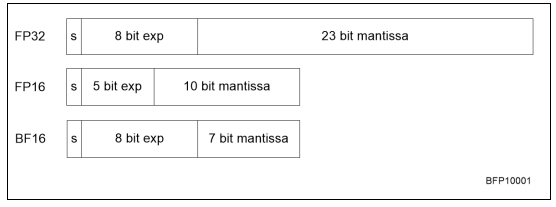
\includegraphics[scale=.5]{bfloat16def}  
  \caption{Comparison of fp32, fp16, and bfloat16
    formats. (Illustration from \cite{Intel:bfloat16}.)}
  \label{fig:bfloat16def}
\end{figure}

\begin{itemize}
\item Since bfloat16 and fp32 have the same structure in the first two bytes,
  a bfloat16 number can be derived from an fp32 number by
  truncating the third and fourth byte. However, rounding may give
  better results in practice.
\item Conversely, casting a bloat16 to fp32 only requires filling the
  final two bytes with zeros.
\end{itemize}

The limited precision of bfloat16 is probably enough to represent
quantities in \indexac{DL} applications, but in order not to lose
further precision it is envisioned that \ac{FMA} hardware uses 32-bit
numbers internally: the product of two bfloat16 number is a regular
32-bit number. In order to compute inner products (which happens as
part of matrix-matrix multiplication in \indexac{DL}), we then need an
\ac{FMA} unit as in figure~\ref{fig:bfloat16fma}.

\begin{figure}[ht]
  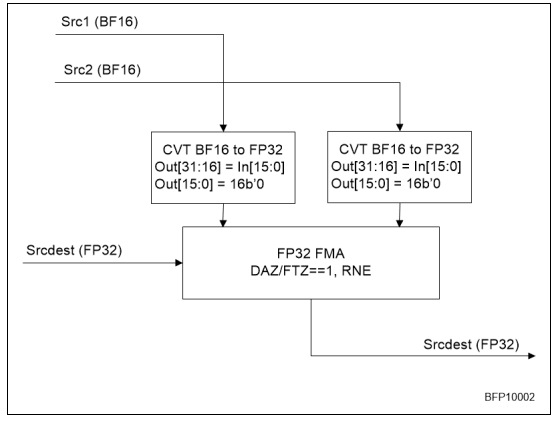
\includegraphics[scale=.5]{bfloat16fma}
  \caption{An FMA unit taking two bloat16 and one fp32
    number. (Illustration from \cite{Intel:bfloat16}.)}
  \label{fig:bfloat16fma}
\end{figure}

\begin{itemize}
\item The 
  \emph{Intel Knights Mill}\index{Intel!Xeon Phi!Knights Mill}, based
  on the \emph{Intel Knights Landing}\index{Intel!Xeon Phi!Knights Landing}, 
  has support for reduced precision.
\item The \indextermbus{Intel}{Cooper Lake} implements the
  \indexterm{bfloat16} format~\cite{Intel:bfloat16}.
\end{itemize}

Even further reduction to 8-bit was discussed in~\cite{dettmers:8bit}.

\Level 1 {Fixed-point arithmetic}

A fixed-point number (for a more thorough discussion than found here,
see~\cite{YatesFixedPoint}) can be represented as $\fxp NF$ where
$N\geq\beta^0$ is the integer part and $F<1$ is the fractional
part. Another way of looking at this, is that a fixed-point number is
an integer stored in $N+F$ digits, with an implied decimal point after
the first $N$ digits.

Fixed-point calculations can overflow, with no possibility to adjust
an exponent. Consider the multiplication $\fxp{N_1}{F_1}\times
\fxp{N_2}{F_2}$, where $N_1\geq \beta^{n_1}$ and $N_2\geq
\beta^{n_2}$. This overflows if $n_1+n_2$ is more than the number of
positions available for the integer part. (Informally, the number of
digits of the product is the sum of the number of digits of the operands.)
This means that, in a program
that uses fixed-point, numbers will need to have a number of
leading zero digits, if you are ever going to multiply them, 
which lowers the numerical accuracy.
It also means that the programmer has to think harder about
calculations, arranging them in such a way that overflow will not
occur, and that numerical accuracy is still preserved to a reasonable
extent.

So why would people use fixed-point numbers? One important application
is in embedded low-power devices, think a battery-powered digital
thermometer. Since fixed-point calculations are essentially identical
to integer calculations, they do not require a floating-point unit,
thereby lowering chip size and lessening power demands. Also, many
early video game systems had a processor that either had no
floating-point unit, or where the integer unit was considerably faster
than the floating-point unit. In both cases, implementing non-integer
calculations as fixed-point, using the integer unit, was the key to
high throughput. 

Another area where fixed point arithmetic is still used is in signal
processing. In modern CPUs, integer and floating point operations
are of essentially the same speed, but converting between them is
relatively slow. Now, if the sine function is implemented through
table lookup, this means that in $\sin(\sin x)$ 
the output of a function is used to index the next function
application. Obviously, outputting the sine function in fixed point
obviates the need for conversion between real and integer quantities,
which simplifies the chip logic needed, and speeds up calculations.

\Level 1 {Complex numbers}
\label{sec:complex}
\index{complex numbers|(}

Some programming languages have \emph{complex numbers} as a built-in data type,
others not, and others are in between. For instance, in Fortran you
can declare
\begin{verbatim}
COMPLEX z1,z2, z(32)
COMPLEX*16 zz1, zz2, zz(36)
\end{verbatim}
A complex number is a pair of real numbers, the real and imaginary
part, allocated adjacent in memory. The first declaration then uses
8~bytes to store to \n{REAL*4} numbers, the second one has \n{REAL*8}s
for the real and imaginary part.  (Alternatively, use \n{DOUBLE
  COMPLEX} or in Fortran90 \n{COMPLEX(KIND=2)} for the second line.)

By contrast, the \n{C} language does not directly have complex
numbers, but both \n{C99} and \n{C++} have a \n{complex.h} header
file
\begin{footnoteenv}
  {These two header files are not identical, and in fact
  not compatible. Beware, if you compile C code with a C++
  compiler~\cite{DobbsComplex}.}
\end{footnoteenv}
. This defines as complex number as in
Fortran, as two real numbers.

Storing a complex number like this is easy, but sometimes it is
computationally not the best solution. This becomes apparent when we
look at arrays of complex numbers.
If a computation often relies
on access to the real (or imaginary) parts of complex numbers
exclusively, striding through an array of complex numbers, has a
stride two, which is disadvantageous (see
section~\ref{sec:stride}). In this case, it is better to allocate one
array for the real parts, and another for the imaginary parts.

\begin{exercise}
  Suppose arrays of complex numbers are stored the Fortran
  way. Analyze the memory access pattern of pairwise multiplying the
  arrays, that is, $\forall_i\colon c_i\leftarrow a_i\cdot b_i$, where
  \texttt{a(), b(), c()} are arrays of complex numbers.
\end{exercise}

\begin{exercise}
  Show that an $n\times n$ linear system $Ax=b$ over the complex numbers
  can be written as a $2n\times 2n$ system over the real
  numbers. Hint: split the matrix and the vectors in their real and
  imaginary parts. Argue for the efficiency of storing arrays of
  complex numbers as separate arrays for the real and imaginary parts.
\end{exercise}

\index{complex numbers|)}

\Level 0 {Conclusions}

Computations done on a computer are invariably beset with numerical error.
In a way, the reason for the error is the imperfection of computer
arithmetic: if we could calculate with actual real numbers there would
be no problem. (There would still be the matter of measurement error
in data, and approximations made in numerical methods; see the next
chapter.) However, if we accept roundoff as a fact of life, then
various observations hold:
\begin{itemize}
\item Mathematically equivalent operations need not behave identically
  from a point of stability; see the `abc-formula' example.
\item Even rearrangements of the same computations do not behave
  identically; see the summing example.
\end{itemize}
Thus it
becomes imperative to analyze computer algorithms with regard to their
roundoff behavior: does roundoff increase as a slowly growing
function of problem parameters, such as the number of terms evaluated,
or is worse behavior possible? We will not address such questions in
further detail in this book.

\index{floating point arithmetic|)}

\Level 0 {Review questions}

\begin{exercise}
  True or false?
  \begin{itemize}
  \item For integer types, the `most negative' integer is the negative
    of the `most positive' integer.
  \item For floating point types, the `most negative' number is the negative
    of the `most positive' one.
  \item For floating point types, the smallest positive number is the reciprocal
    of the largest positive number.
  \end{itemize}
\end{exercise}

% LocalWords:  Eijkhout textbf Overton Higham imod bitstrings gcc Inf
% LocalWords:  bitstring bitshift bitshifts leftshift rightshift NaN
% LocalWords:  significand denormalized typename IEC MATLAB's Cleve
% LocalWords:  Moler Kahan endian NVidia Tesla LBM FMA sizeof
% LocalWords:  datatype
